\documentclass[a4paper]{article}

\usepackage[english]{babel}
\usepackage[utf8]{inputenc}
\usepackage{amsmath}
\usepackage{graphicx}
\usepackage[colorinlistoftodos]{todonotes}
\usepackage{pdfpages}

\title{InfoEmb TP2}

\author{Jérôme Skoda}

\date{\today}

\begin{document}
\maketitle

\begin{abstract}
 Colimaçon: \newline
 001  002  003  004  005  006  007  008  009  010 \newline
 022  023  024  025  026  027  028  029  030  011 \newline
 021  020  019  018  017  016  015  014  013  012 \newline
\end{abstract}

\section{Comment compiler le projet}

\begin{itemize}
\item make all: Compile tout les fichiers
\item make test: Lancement de la série de tests automatiques
\item make lib: Génération de la bibliothéque static et dynamique
\item make doc: Génération de la documentation (doxygen)
\item make rapport: Génération du rapport (latex)
\item make clean: Nettoyage du projet (supression des objets et binaires)
\item make demo-1 ligne=X col=X: Lancer la démo colimacon
\item make demo-2: Lancer la démo horizontal
\item make demo-3: Lancer la démo vertical
\item make demo-4: Lancer la démo carré
\item make demo-5 ligne=X col=X: Lancer la démo colimacon sans print (utile pour le bench)
\item make demo-6 ligne=X col=X: Lancer la démo colimacon avec sortie temps (utile pour le bench)
\end{itemize}

\section{Arborescence}

\begin{itemize}
\item bin : Binaire exécutable
\begin{itemize}
  \item demo : Exécutable de démonstration
  \item test : Exécutable de test
\end{itemize}
\item lib : Bibliothéque
\item doc : Documentation doxygen sous differents formats
\item rapport : Source du rapport
\item res : Ressources necessaire au projet (fichier de bdd)
\item script  : Script utilisé pour les test
\item src : Source du projet
\begin{itemize}
  \item colimacon : Source de colimacon
  \item demo  : Sources des differentes démonstrations d'utilisation
  \item test  : Sources des dufferents tests
\end{itemize}

\item sujet.pdf  : Sujet du projet
\item README.md  : Le readme du projet 
\item rappot.pdf : C'est moi
\end{itemize}

\section{Test disponible}
Les test fonctione de la manière suivante: un script bash exécute chacun de binaire de 
test un par un en enregistrant le sortie standard dans un fichier .out 
Ensuite il compare avec la commande diff chacun des fichier .out avec la 
valeur attendu dont la valeur est stoqué dans un fichier .expected

Les fichier .out et .expected sont dans le répertoire src/test/ 
Le script se situe dans le repertoire script

Les test disponible sont:
\begin{itemize}
  \item  colimacon 1x1
  \item  colimacon 1x10
  \item  colimacon 10x1
  \item  colimacon 10x2
  \item  colimacon 2x10
  \item  colimacon 10x10
  \item  colimacon 1000x1000 (sans print)
\end{itemize}


\section{Fonctionnement}

Le remplissage s'effectue avec un systeme de borne (voir struct borne) et de séquence de direction (voir direction\_t).

Chacune des écriture sont faite dans un ordre de direction: DROITE puis BAS puis GAUCHE puis HAUT jusqu'à que le tableau soit remplis.

L'écriture dans une direction fonctionne de cette manière suivante:
\begin{itemize}
  \item On calcule la position inital du curseur en fonction des borne et de la direction. (\_get\_position\_initiale)
  \item On regarde si l'on peux ecrire dans la case calculé (\_canWrite)
  \item S'il est possible d'écrire, on le fait puis on réitére l'operation en avançant le curseur d'une case à chaque fois (\_iter\_curseur) 
  \item Enfin quand l'écriture n'est plus possible, on avance la borne en fonction de la direction d'écriture (\_iter\_borne) et l'on passe à la direction suivante
\end{itemize}

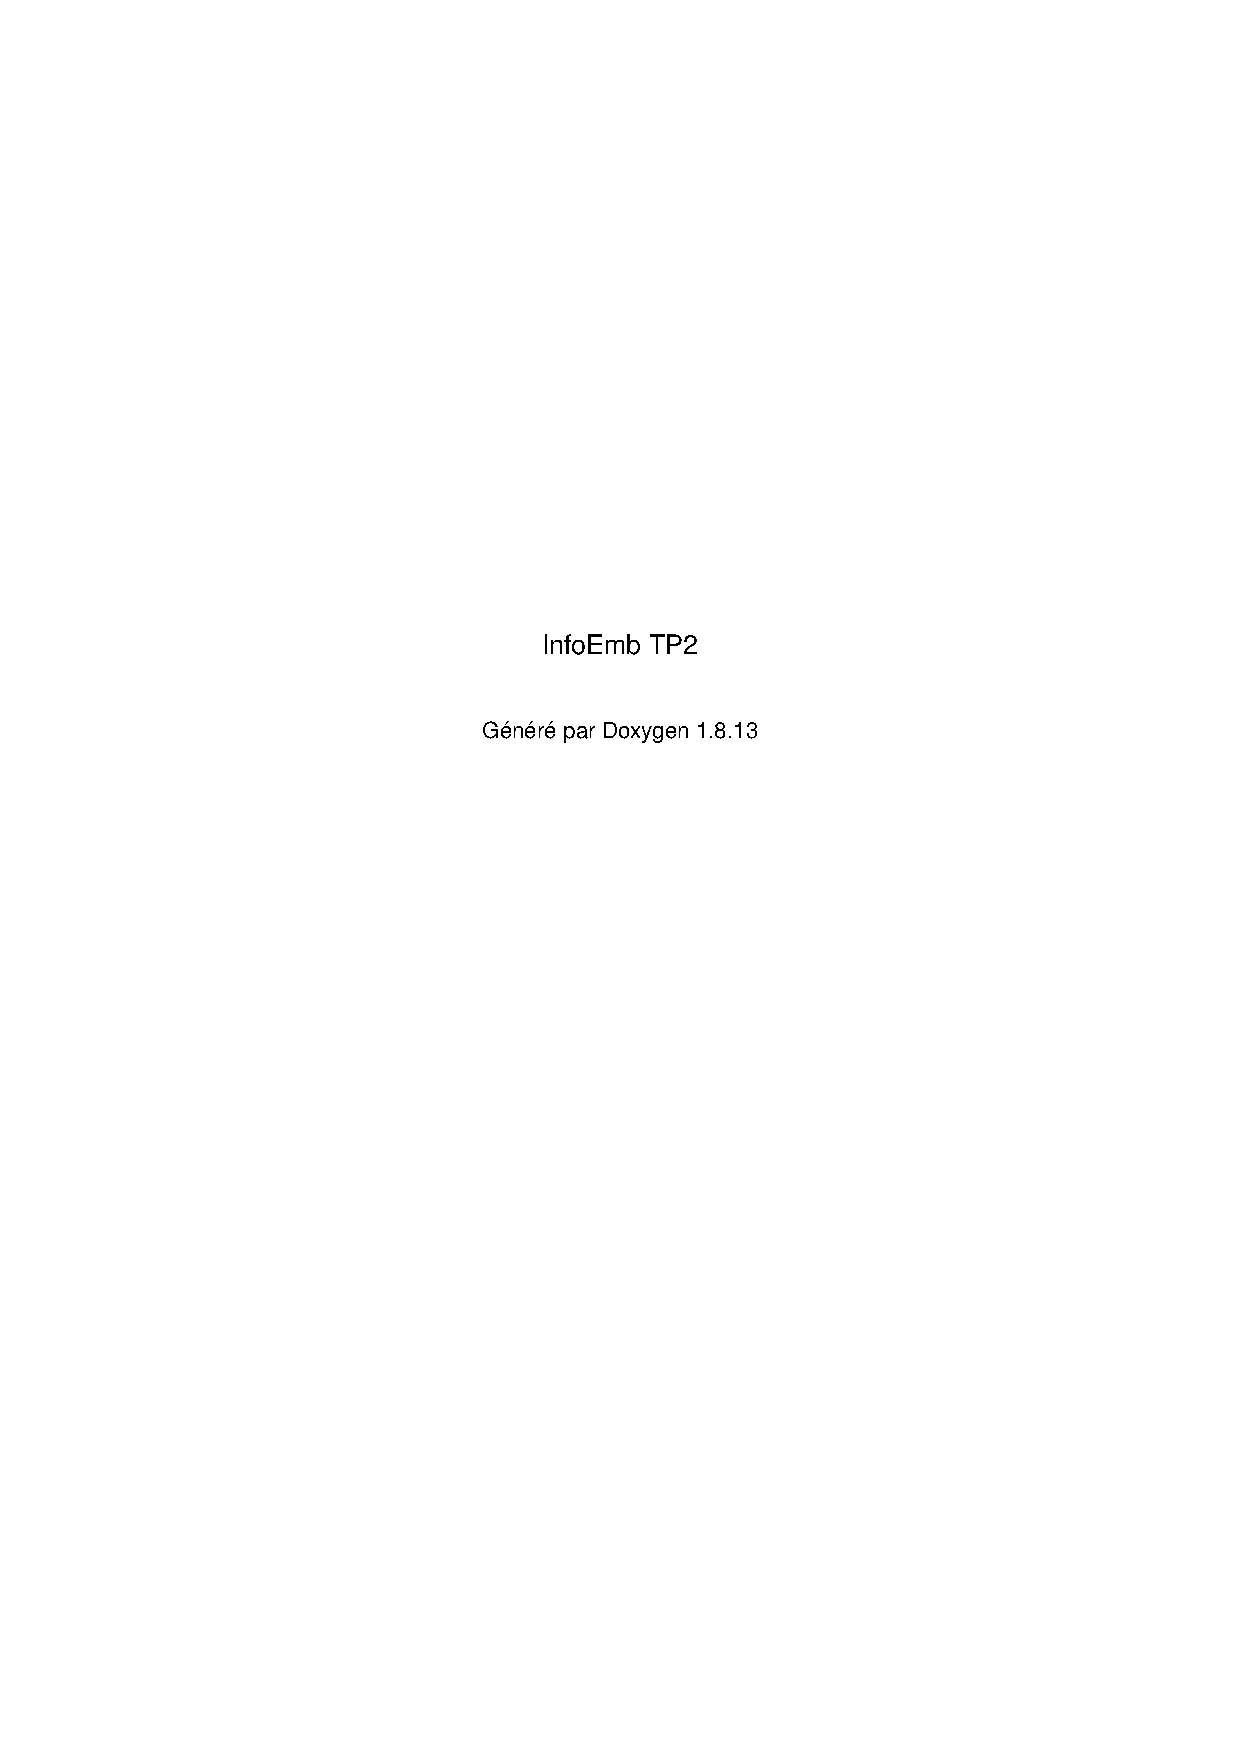
\includepdf[pages=1-15]{refman.pdf}

\end{document}
              
